\documentclass[11pt,a4paper]{article}

\usepackage[utf8]{inputenc}
\usepackage[T1]{fontenc}
\usepackage[spanish]{babel}
\usepackage{geometry}
\usepackage{graphicx}
\usepackage{booktabs}
\usepackage{amsmath}
\usepackage{float}
\usepackage{caption}
\usepackage{array}
\usepackage{hyperref}

\geometry{left=1.8 cm,right=2.2cm,top=2.2cm,bottom=1.8 cm}
\setlength{\parskip}{0.45em}
\setlength{\parindent}{0pt}
\captionsetup{font=small}

\title{Pronóstico de demanda eléctrica diaria en Gran Buenos Aires mediante modelos ARIMA, SARIMA y SARIMAX}

\author{
Jorge Adrián Alvarez \\
Nahuel Elias de la Paz Otonelo Canale \\
\\
Análisis de Series de Tiempo \\
Especialización en Inteligencia Artificial -- FIUBA
}
\usepackage{xurl}
\usepackage{hyperref}
\hypersetup{
    colorlinks=true,
    linkcolor=black,
    urlcolor=blue,
    citecolor=black
}
\date{Junio de 2026}

\begin{document}

\maketitle

\section{Introducción y pregunta de investigación}

Este trabajo analiza la serie de demanda neta diaria de energía eléctrica de la región Gran Buenos Aires (GBA), expresada en MWh, junto con la temperatura media diaria de referencia para la misma región, expresada en grados Celsius. Los datos fueron trabajados a partir del archivo \texttt{Base\_Demanda\_ Diaria\_2017\_2026.xlsx}, hoja \texttt{Datos\_Region}. En el notebook se indica que la base corresponde a información histórica de demanda neta diaria del MEM entre enero de 2017 y abril de 2026, consolidada a partir de mediciones comerciales. \footnote{CAMMESA: comportamiento de la demanda de energía eléctrica en el MEM''. Disponible en: \url{https://cammesaweb.cammesa.com/2026/06/12/covid-19-comportamiento-de-la-demanda-de-energia-electrica-en-el-mem/}}. La variable de demanda utilizada corresponde a la columna \texttt{GRAN BS.AS.}; la temperatura corresponde a \texttt{TEMPERATURA REFERENCIA MEDIA GBA °C}.

La pregunta de investigación propuesta es: \emph{¿en qué medida la incorporación de estructura estacional semanal y temperatura media diaria mejora el pronóstico de la demanda eléctrica diaria de Gran Buenos Aires respecto de un modelo ARIMA no estacional?}

Para responderla se comparan cuatro familias de modelos: ARIMA, SARIMA, SARIMAX con temperatura y SARIMAX con temperatura centrada y término cuadrático. El entrenamiento se realizó con datos desde 2017 hasta 2024, y la evaluación fuera de muestra se realizó sobre el período 2025--2026 disponible.

\begin{figure}[H]
\centering
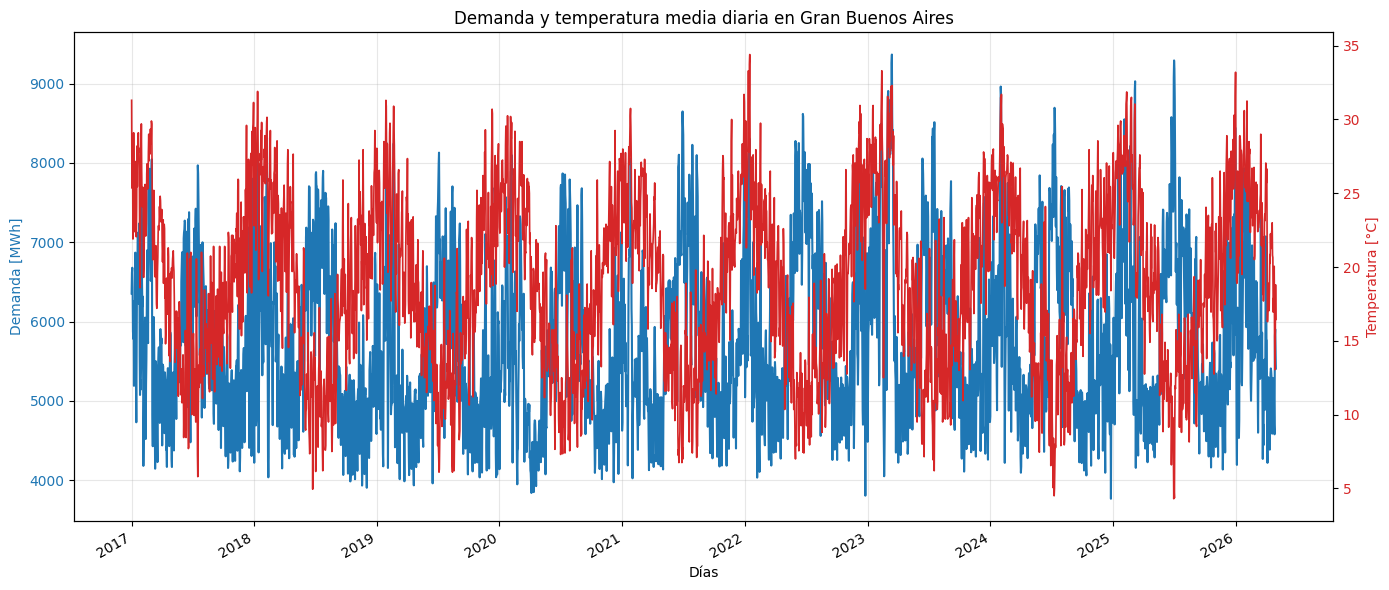
\includegraphics[width=0.92\textwidth]{informe_figuras/serie_completa_demanda_temperatura.png}
\caption{Serie completa de demanda diaria y temperatura media diaria en Gran Buenos Aires.}
\label{fig:serie_completa}
\end{figure}

\section{Análisis exploratorio y estacionariedad}

La Figura \ref{fig:serie_completa} muestra que la demanda presenta variabilidad de corto plazo, cambios de nivel y patrones estacionales. Para observar mejor el período usado como test, la Figura \ref{fig:serie_2025} muestra el detalle desde 2025. En ese tramo se observan picos de demanda y oscilaciones regulares que no son capturables mediante un modelo puramente constante en media.

\begin{figure}[H]
\centering
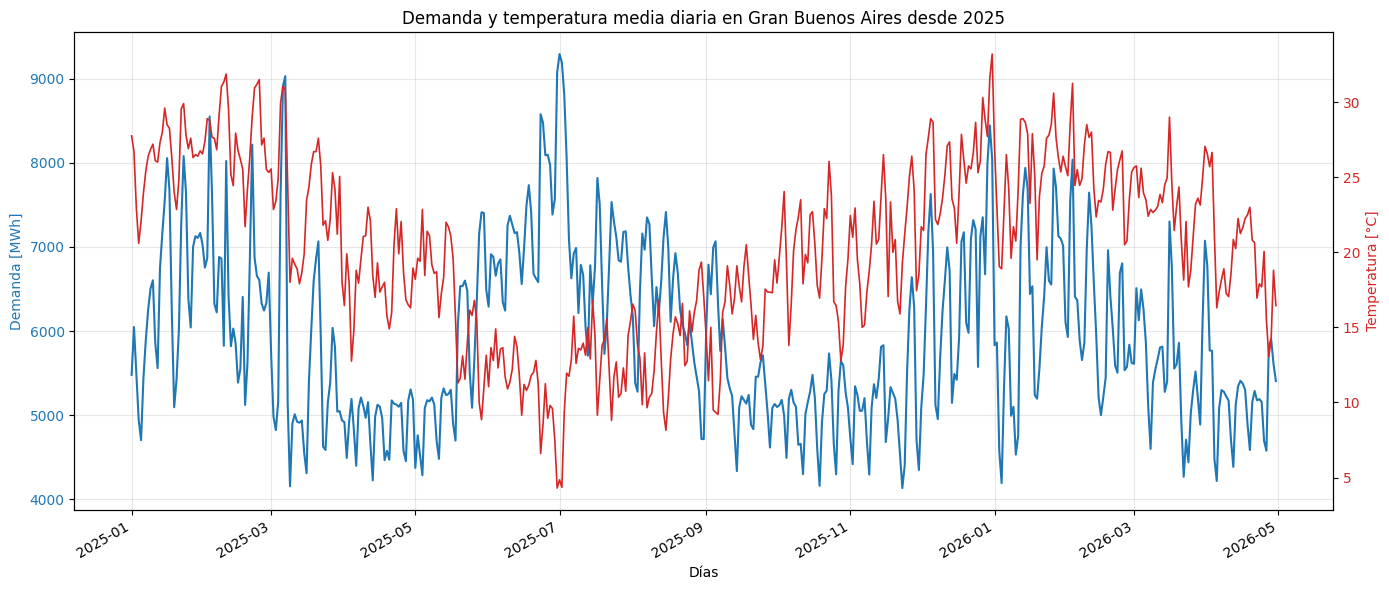
\includegraphics[width=0.92\textwidth]{informe_figuras/serie_2025_2026_demanda_temperatura.png}
\caption{Detalle de demanda y temperatura media diaria desde 2025.}
\label{fig:serie_2025}
\end{figure}

Como análisis exploratorio adicional se aplicó una descomposición MSTL con períodos 7 y 365. Esta descomposición permitió identificar una componente semanal clara y una componente anual de mayor amplitud, aunque menos suave. La componente semanal se interpreta como evidencia de diferencias sistemáticas entre días de la semana, mientras que la componente anual se vincula con variaciones de temperatura y calendario. 

\begin{figure}[H]
\centering
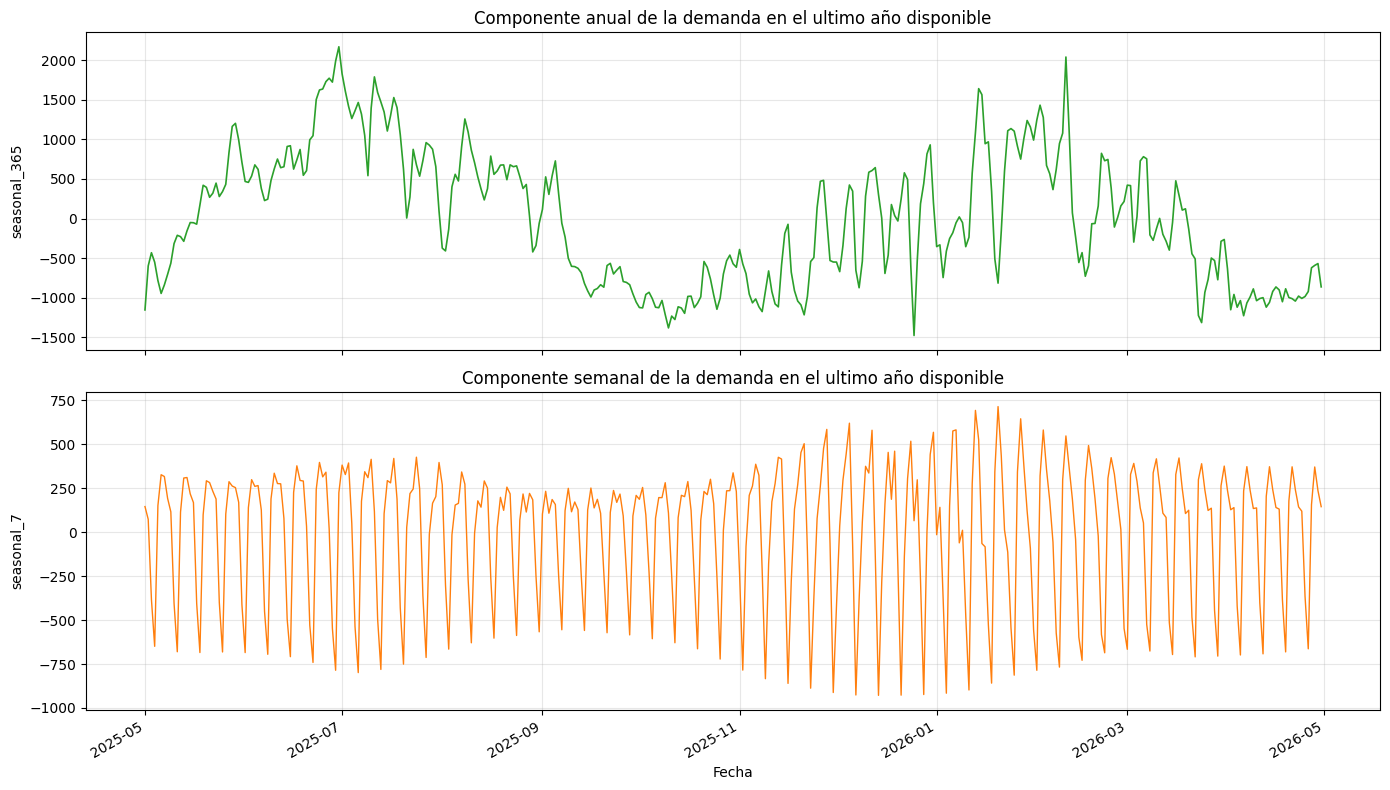
\includegraphics[width=0.88\textwidth]{informe_figuras/componentes_estacionales_ultimo_anio.png}
\caption{Componentes estacionales semanal y anual en el último año disponible.}
\label{fig:mstl}
\end{figure}

Luego se aplicó la prueba ADF sobre la serie diaria regularizada. La hipótesis nula de esta prueba es la presencia de raíz unitaria. El estadístico obtenido fue:
\[
ADF=-6.153,\qquad p\text{-value}=7.48\times 10^{-8}.
\]
Dado que el valor-p es menor que 0.05, se rechaza la hipótesis nula y se considera que hay evidencia de estacionariedad en nivel. Por este motivo, en las especificaciones iniciales se tomó \(d=0\). Sin embargo, la estacionariedad en nivel no elimina la presencia de dependencia temporal ni de estacionalidad semanal.

Los gráficos ACF y PACF de la Figura \ref{fig:acf_pacf} muestran dependencia temporal significativa. La ACF mantiene valores relevantes durante varios rezagos y presenta señales en múltiplos de 7 días. La PACF muestra un pico dominante en el rezago 1, lo que sugiere una componente autorregresiva de corto plazo. Estos elementos justifican comenzar con un ARIMA de bajo orden y luego avanzar hacia modelos con estructura estacional semanal.

\begin{figure}[H]
\centering
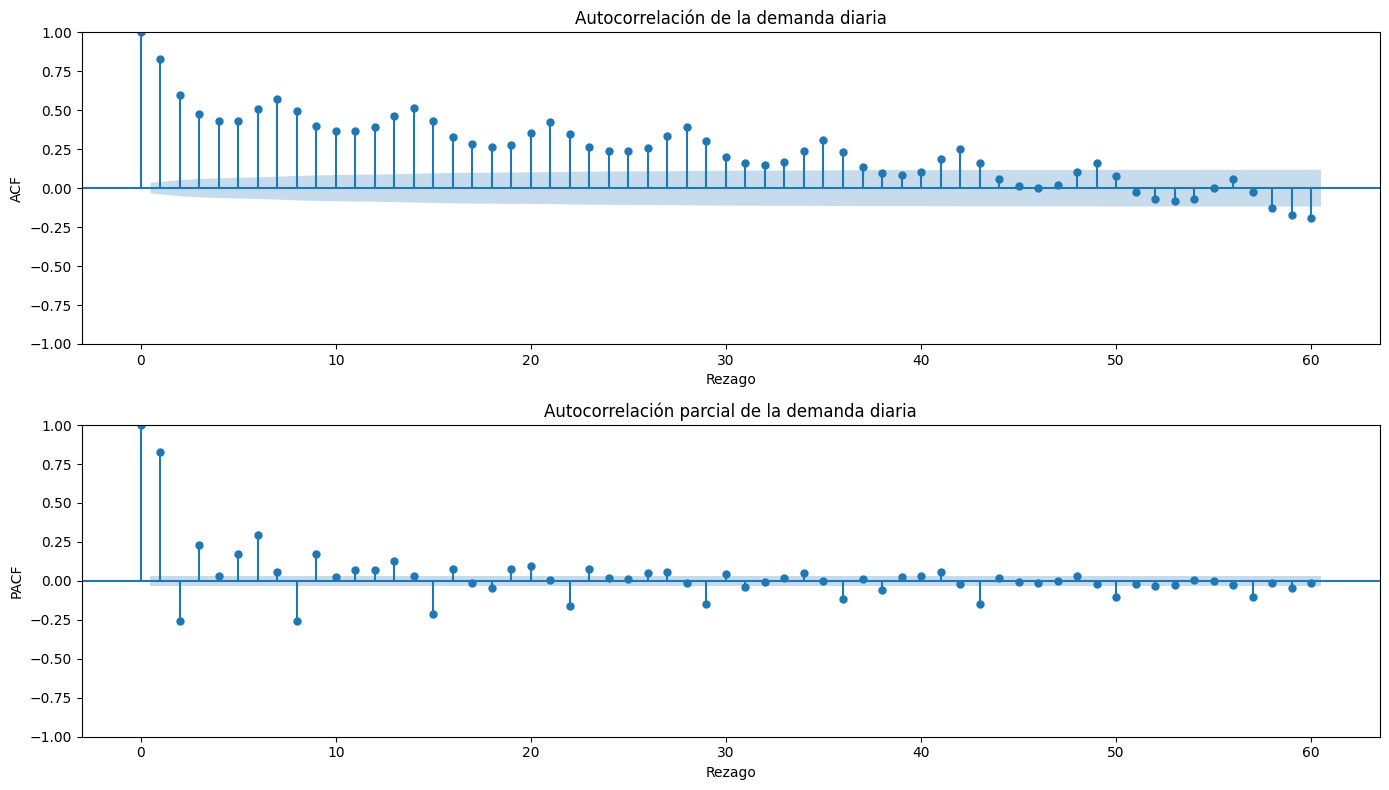
\includegraphics[width=0.88\textwidth]{informe_figuras/acf_pacf_demanda.png}
\caption{Autocorrelación y autocorrelación parcial de la demanda diaria.}
\label{fig:acf_pacf}
\end{figure}

\section{Modelos propuestos}

El primer modelo considerado fue un ARIMA no estacional:
\[
\phi(L)(Y_t-\mu)=\theta(L)\varepsilon_t,
\]
donde \(Y_t\) representa la demanda diaria y \(\varepsilon_t\) es el error del modelo. A partir de la comparación de órdenes bajos, se utilizó como referencia el modelo ARIMA(2,0,2). Este modelo captura dependencia temporal de corto plazo, pero no incorpora explícitamente la estacionalidad semanal.

El segundo modelo fue un SARIMA con período semanal:
\[
\Phi(L^7)\phi(L)(1-L^7)^D(Y_t-\mu)=\Theta(L^7)\theta(L)\varepsilon_t.
\]
En el notebook se ajustó un modelo con estructura semanal \(s=7\), tomando la estacionalidad semanal observada en la ACF y en la descomposición exploratoria.

El tercer modelo incorporó temperatura media diaria como variable exógena:
\[
Y_t = m_t + \beta_1 T_t + \varepsilon_t,
\]
donde \(m_t\) sigue una estructura SARIMA y \(T_t\) es la temperatura media diaria. La motivación es que parte de la demanda puede estar asociada a condiciones térmicas, especialmente por consumo relacionado con calefacción o refrigeración.

Finalmente, se consideró una especificación no lineal en temperatura:
\[
Y_t = m_t + \beta_1 T_{c,t} + \beta_2 T_{c,t}^{2}+\varepsilon_t,
\qquad
T_{c,t}=T_t-\bar T_{\text{train}}.
\]
El centrado de la temperatura se realizó usando la media del conjunto de entrenamiento. Esta transformación permite modelar una relación no lineal entre demanda y temperatura y reduce problemas numéricos entre \(T_t\) y \(T_t^2\).

\section{Resultados de pronóstico}

Las Figuras \ref{fig:arima_sarima} y \ref{fig:sarimaxs} comparan los pronósticos fuera de muestra de los cuatro modelos frente a la demanda observada en el período de test. El ARIMA(2,0,2) queda cerca de un nivel medio y no reproduce la variabilidad diaria ni la estacionalidad semanal. El SARIMA introduce una oscilación semanal más clara, aunque su pronóstico resulta todavía demasiado regular y no acompaña adecuadamente los cambios de nivel.

\begin{figure}[H]
\centering
\begin{minipage}{0.49\textwidth}
\centering
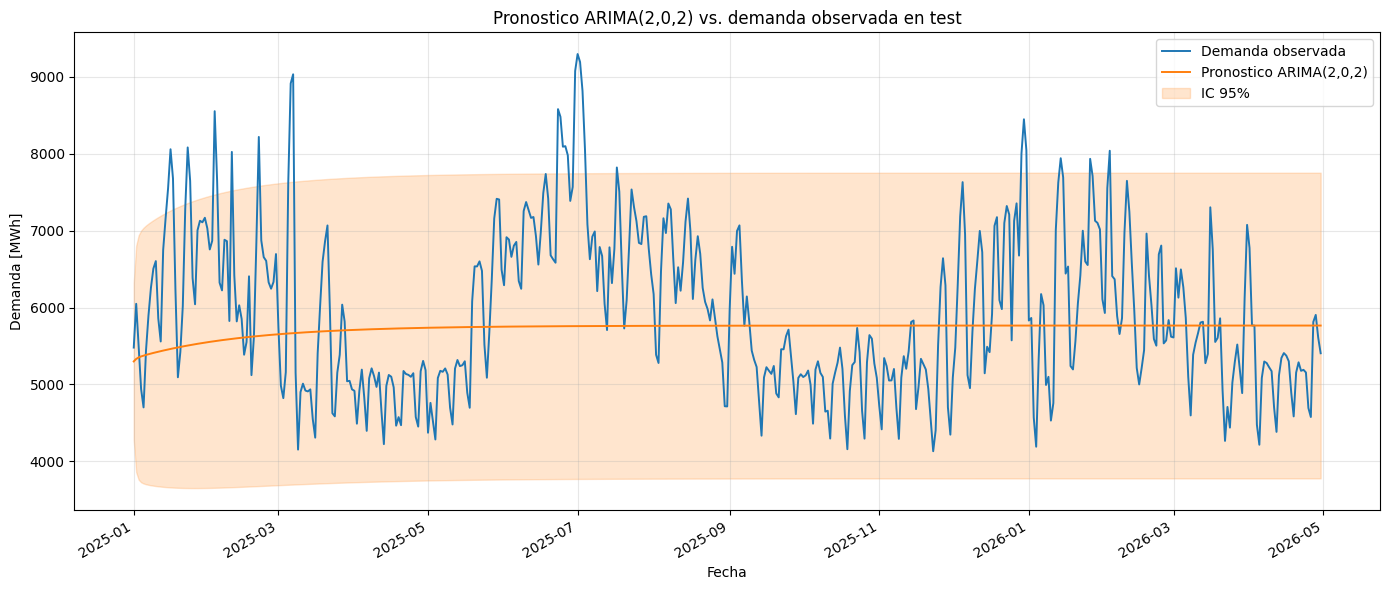
\includegraphics[width=\textwidth]{informe_figuras/pronostico_arima.png}
\caption*{ARIMA(2,0,2)}
\end{minipage}
\hfill
\begin{minipage}{0.49\textwidth}
\centering
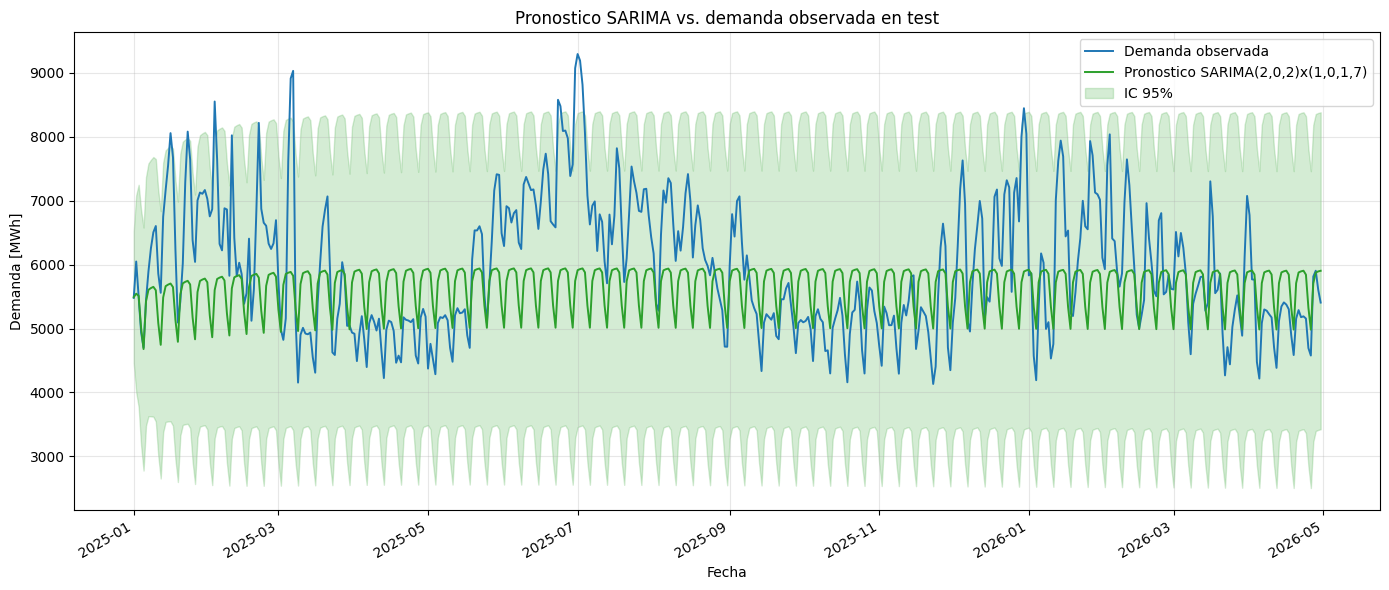
\includegraphics[width=\textwidth]{informe_figuras/pronostico_sarima.png}
\caption*{SARIMA semanal}
\end{minipage}
\caption{Pronósticos de los modelos ARIMA y SARIMA.}
\label{fig:arima_sarima}
\end{figure}

El SARIMAX con temperatura mejora levemente el comportamiento respecto de los modelos univariados, pero todavía no reproduce adecuadamente los picos de la serie. El modelo SARIMAX con temperatura centrada y término cuadrático logra seguir mejor los cambios de nivel y reduce visualmente la distancia con la serie observada. Aun así, persisten errores en picos extremos y períodos de alta volatilidad.

\begin{figure}[H]
\centering
\begin{minipage}{0.49\textwidth}
\centering
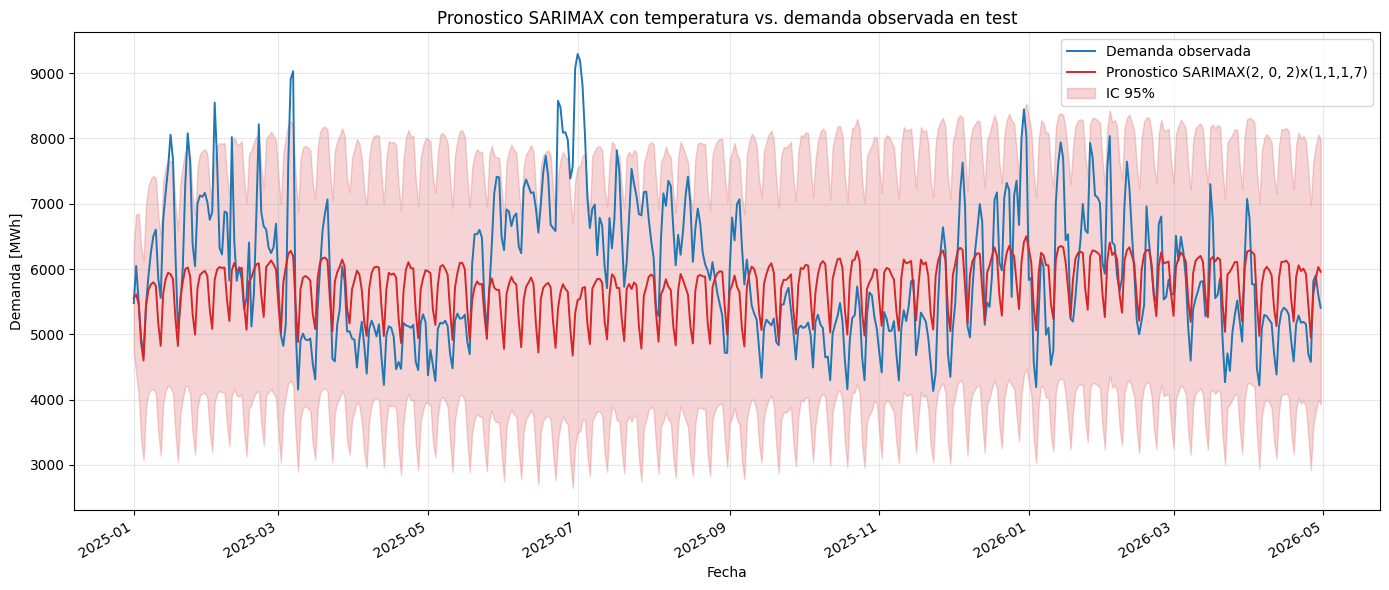
\includegraphics[width=\textwidth]{informe_figuras/pronostico_sarimax_temp.png}
\caption*{SARIMAX con temperatura}
\end{minipage}
\hfill
\begin{minipage}{0.49\textwidth}
\centering
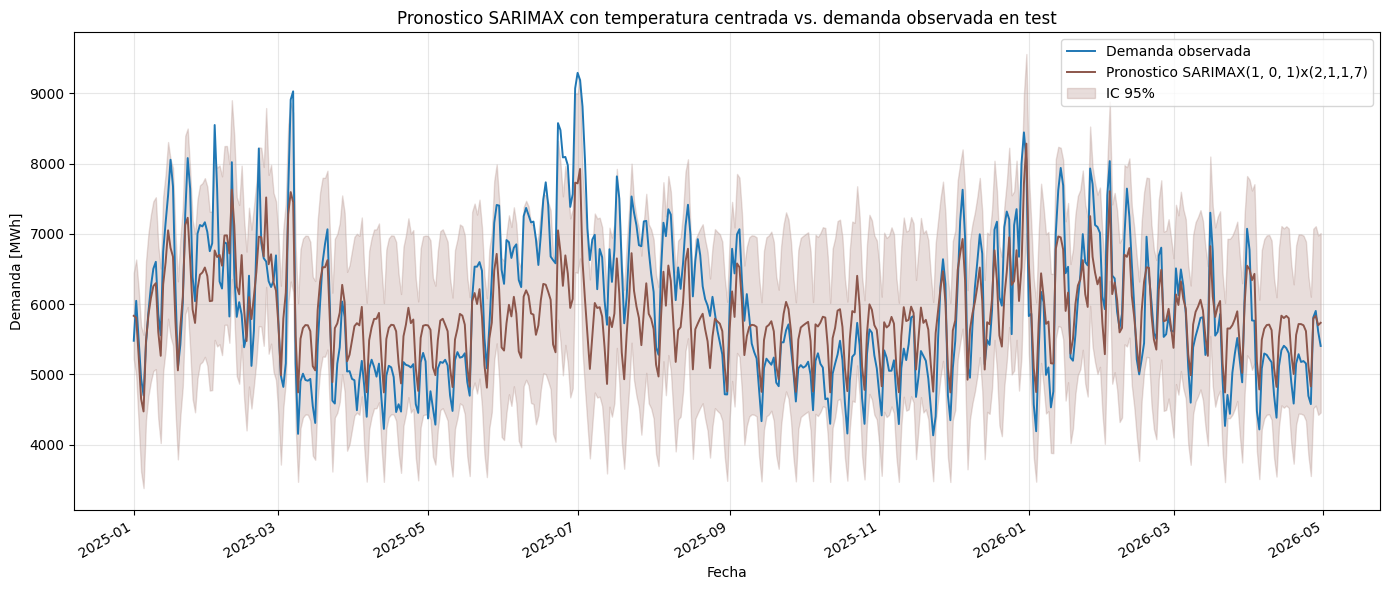
\includegraphics[width=\textwidth]{informe_figuras/pronostico_sarimax_temp_cuadratica.png}
\caption*{SARIMAX con \(T_c\) y \(T_c^2\)}
\end{minipage}
\caption{Pronósticos de los modelos SARIMAX con variables exógenas de temperatura.}
\label{fig:sarimaxs}
\end{figure}

La Tabla \ref{tab:metricas} resume las métricas de evaluación sobre el conjunto de test. Se reportan MAE, RMSE y MAPE. El MAE y el RMSE están expresados en MWh, mientras que el MAPE se expresa en porcentaje. También se incluye el AIC de entrenamiento como referencia de ajuste in-sample, aunque la selección final se realiza priorizando el desempeño fuera de muestra.

\begin{table}[H]
\centering
\small
\begin{tabular}{lrrrr}
\toprule
Modelo & AIC & MAE & RMSE & MAPE \\
\midrule
ARIMA(2,0,2) & 44852.37 & 881.69 & 1082.04 & 14.53 \\
SARIMA semanal & 43543.59 & 839.615 & 1033.315 & 13.525 \\
SARIMAX + \(T_t\) & 43227.25 & 845.309 & 1032.369 & 13.811 \\
SARIMAX + \(T_c,T_c^2\) & 41564.79 & 568.234 & 699.235 & 9.238  \\
\bottomrule
\end{tabular}
\caption{Comparación de métricas de pronóstico sobre el conjunto de test.}
\label{tab:metricas}
\end{table}

\section{Conclusiones}

El análisis muestra que la demanda diaria de GBA tiene dependencia temporal, estructura semanal y una relación relevante con la temperatura. El ARIMA(2,0,2) sirve como modelo base no estacional, pero su pronóstico tiende a estabilizarse alrededor de un nivel medio y no logra capturar la dinámica observada. La incorporación de estacionalidad semanal mediante SARIMA mejora el ajuste, aunque el pronóstico continúa siendo demasiado regular.

Los modelos SARIMAX incorporan información externa de temperatura. El modelo con temperatura lineal mejora levemente las métricas respecto del SARIMA, pero el salto más importante se observa al incluir temperatura centrada y su término cuadrático. Este último modelo reduce el MAPE de 14.53\% en ARIMA a 9.39\%, y también disminuye de forma marcada el MAE y el RMSE. Por lo tanto, entre los modelos evaluados, el mejor candidato predictivo es el SARIMAX con \(T_c\) y \(T_c^2\).

Cabe remarcar que durante el ajuste de los modelos SARIMAX se observaron advertencias de no convergencia. Para resolver este problema se incrementó el número máximo de iteraciones del algoritmo de optimización mediante el parámetro maxiter=1000. Luego de esta modificación, todos los modelos estimados convergieron correctamente.
\end{document}
